% Options for packages loaded elsewhere
\PassOptionsToPackage{unicode}{hyperref}
\PassOptionsToPackage{hyphens}{url}
%
\documentclass[
  ignorenonframetext,
]{beamer}
\usepackage{pgfpages}
\setbeamertemplate{caption}[numbered]
\setbeamertemplate{caption label separator}{: }
\setbeamercolor{caption name}{fg=normal text.fg}
\beamertemplatenavigationsymbolsempty
% Prevent slide breaks in the middle of a paragraph
\widowpenalties 1 10000
\raggedbottom
\setbeamertemplate{part page}{
  \centering
  \begin{beamercolorbox}[sep=16pt,center]{part title}
    \usebeamerfont{part title}\insertpart\par
  \end{beamercolorbox}
}
\setbeamertemplate{section page}{
  \centering
  \begin{beamercolorbox}[sep=12pt,center]{part title}
    \usebeamerfont{section title}\insertsection\par
  \end{beamercolorbox}
}
\setbeamertemplate{subsection page}{
  \centering
  \begin{beamercolorbox}[sep=8pt,center]{part title}
    \usebeamerfont{subsection title}\insertsubsection\par
  \end{beamercolorbox}
}
\AtBeginPart{
  \frame{\partpage}
}
\AtBeginSection{
  \ifbibliography
  \else
    \frame{\sectionpage}
  \fi
}
\AtBeginSubsection{
  \frame{\subsectionpage}
}
\usepackage{amsmath,amssymb}
\usepackage{iftex}
\ifPDFTeX
  \usepackage[T1]{fontenc}
  \usepackage[utf8]{inputenc}
  \usepackage{textcomp} % provide euro and other symbols
\else % if luatex or xetex
  \usepackage{unicode-math} % this also loads fontspec
  \defaultfontfeatures{Scale=MatchLowercase}
  \defaultfontfeatures[\rmfamily]{Ligatures=TeX,Scale=1}
\fi
\usepackage{lmodern}
\ifPDFTeX\else
  % xetex/luatex font selection
\fi
% Use upquote if available, for straight quotes in verbatim environments
\IfFileExists{upquote.sty}{\usepackage{upquote}}{}
\IfFileExists{microtype.sty}{% use microtype if available
  \usepackage[]{microtype}
  \UseMicrotypeSet[protrusion]{basicmath} % disable protrusion for tt fonts
}{}
\makeatletter
\@ifundefined{KOMAClassName}{% if non-KOMA class
  \IfFileExists{parskip.sty}{%
    \usepackage{parskip}
  }{% else
    \setlength{\parindent}{0pt}
    \setlength{\parskip}{6pt plus 2pt minus 1pt}}
}{% if KOMA class
  \KOMAoptions{parskip=half}}
\makeatother
\usepackage{xcolor}
\newif\ifbibliography
\usepackage{graphicx}
\makeatletter
\newsavebox\pandoc@box
\newcommand*\pandocbounded[1]{% scales image to fit in text height/width
  \sbox\pandoc@box{#1}%
  \Gscale@div\@tempa{\textheight}{\dimexpr\ht\pandoc@box+\dp\pandoc@box\relax}%
  \Gscale@div\@tempb{\linewidth}{\wd\pandoc@box}%
  \ifdim\@tempb\p@<\@tempa\p@\let\@tempa\@tempb\fi% select the smaller of both
  \ifdim\@tempa\p@<\p@\scalebox{\@tempa}{\usebox\pandoc@box}%
  \else\usebox{\pandoc@box}%
  \fi%
}
% Set default figure placement to htbp
\def\fps@figure{htbp}
\makeatother
\setlength{\emergencystretch}{3em} % prevent overfull lines
\providecommand{\tightlist}{%
  \setlength{\itemsep}{0pt}\setlength{\parskip}{0pt}}
\setcounter{secnumdepth}{-\maxdimen} % remove section numbering
\definecolor{burntorange}{rgb}{0.968, 0.549, 0.114}
\definecolor{burntorangedark}{rgb}{0.486, 0.306, 0.102}
\definecolor{lightblue}{rgb}{0.161, 0.471, 1}
\definecolor{lightbluedark}{rgb}{0.125, 0.271, 0.510}
\definecolor{charcoal}{rgb}{0.21, 0.27, 0.31}
\definecolor{darkgray}{rgb}{0.3, 0.3, 0.3}
\definecolor{darkgrey}{rgb}{0.33, 0.33, 0.33}
\definecolor{cadmiumgreen}{rgb}{0.0, 0.42, 0.24}
\definecolor{brandeisblue}{rgb}{0.0, 0.44, 1.0}
\setbeamercolor{structure}{fg=darkgray}
\setbeamercolor{footline}{fg=darkgray}
\usepackage{amssymb, bm}
\usepackage{amsmath, amsfonts, amscd, epsfig, amssymb, amsthm, adjustbox}
\usepackage{textcomp}
\usepackage{graphicx}
\usepackage{setspace}
\usepackage{enumitem}
\setlist[itemize]{itemsep=9pt, label={--}}
\usepackage{anyfontsize}
\usepackage{ulem}
\usepackage{tcolorbox}[most]
\usepackage{tikz}
\usepackage[T1]{fontenc}
\usepackage{booktabs}
\usepackage{soul}
\setul{4.5pt}{3pt} % First value is thickness, second is distance from text
\usepackage{colortbl}
\usepackage{multirow}
\usepackage{array}
\usepackage{longtable}
\usepackage{listings}
\usepackage{color}
\usepackage{bbold}
\usepackage{mathtools}
\newcolumntype{K}[1]{>{\centering\arraybackslash}p{#1}}
\newcolumntype{Q}[1]{>{\columncolor[gray]{0.8}\centering\arraybackslash}p{#1}}
\newcommand\eho{\stackrel{\mathclap{\small\mbox{$H_0$}}}{=}}
\newcommand\norm[1]{\left\lVert#1\right\rVert}
\newcommand\smalldp{\fontsize{9.4}{7.2}\selectfont}
\newcommand\smalldpp{\fontsize{8.5}{7.2}\selectfont}
\newcommand\smalldppgh{\fontsize{9.5}{7.2}\selectfont}
\newcolumntype{H}{>{\setbox0=\hbox\bgroup}c<{\egroup}@{}}
\newcommand{\bo}[1]{\textcolor{burntorange}{#1}}
\newcommand{\bod}[1]{\textcolor{burntorangedark}{#1}}
\newcommand{\lb}[1]{\textcolor{lightblue}{#1}}
\newcommand{\lbd}[1]{\textcolor{lightbluedark}{#1}}
\newcommand{\dg}[1]{\textcolor{darkgray}{#1}}
\newcommand{\bi}{\begin{itemize}}
\newcommand{\ib}{\end{itemize}}
\newcommand{\p}{\item}
\newcommand{\sk}{\vspace{.5cm}}
\newcommand{\sko}{\vspace{.1in}}
\newcommand{\skoo}{\vspace{.2in}}
\newcommand{\skooo}{\vspace{.3in}}
\newcommand{\skoooo}{\vspace{.05in}}
\newcommand{\hko}{\hspace{.1in}}
\newcommand{\hkoo}{\hspace{.2in}}
\newcommand{\hkooo}{\hspace{.3in}}
\newcommand{\bb}{$\lb{{\small \bullet } }$ \hspace{0.5mm}}
\newcommand{\ba}{$\lb{{\small \rightarrow } }$ \hspace{0.5mm}}
\setbeamertemplate{footline}{\scriptsize{\hfill\insertframenumber\vspace{-.2cm}\hspace*{.35cm}}}
\usepackage{bookmark}
\IfFileExists{xurl.sty}{\usepackage{xurl}}{} % add URL line breaks if available
\urlstyle{same}
\hypersetup{
  pdftitle={Constructing Quantitative Arguments},
  pdfauthor={(\textbackslash text\{Professor Dave\})\^{}2},
  hidelinks,
  pdfcreator={LaTeX via pandoc}}

\title{Constructing Quantitative Arguments}
\author{\((\text{Professor Dave})^2\)}
\date{}
\institute{The University of Austin}

\begin{document}
\frame{\titlepage}

\begin{frame}{}
\phantomsection\label{section}
\vspace{.5cm}
\Large \textcolor{darkgray}{You are confronted with a difficult question with many moving parts and possible outcomes.}

\vspace{.5cm}\vspace{.5cm}

How do you effectively answer this question, acknowledging the
complexity, uncertainty, and trade offs involved?
\end{frame}

\begin{frame}{}
\phantomsection\label{section-1}
\vspace{.5cm}
\Large

Are medical schools discriminatory in admissions?
\end{frame}

\begin{frame}{}
\phantomsection\label{section-2}
\vspace{.5cm}
\Large

Are police racist?
\end{frame}

\begin{frame}{}
\phantomsection\label{section-3}
\vspace{.5cm}
\Large

Is private space travel the best way to become a multiplanetary species?
\end{frame}

\begin{frame}{}
\phantomsection\label{section-4}
\vspace{.5cm}
\Large

Is the stock market predictable, and if so, to what degree?
\end{frame}

\begin{frame}{}
\phantomsection\label{section-5}
\vspace{.5cm}
\Large

Will increasing the minimum wage help or hurt the economy?
\end{frame}

\begin{frame}{}
\phantomsection\label{section-6}
\vspace{.5cm}
\Large

Is this vaccine safe and effective?
\end{frame}

\begin{frame}{}
\phantomsection\label{section-7}
\vspace{.5cm}
\Large

Should I propose to a fellow UATX student?
\end{frame}

\begin{frame}{}
\phantomsection\label{section-8}
\vspace{.5cm}
\Large

Should I \st{propose to} ask out a fellow UATX student?
\end{frame}

\begin{frame}{An analogy: Building a house}
\phantomsection\label{an-analogy-building-a-house}
\pandocbounded{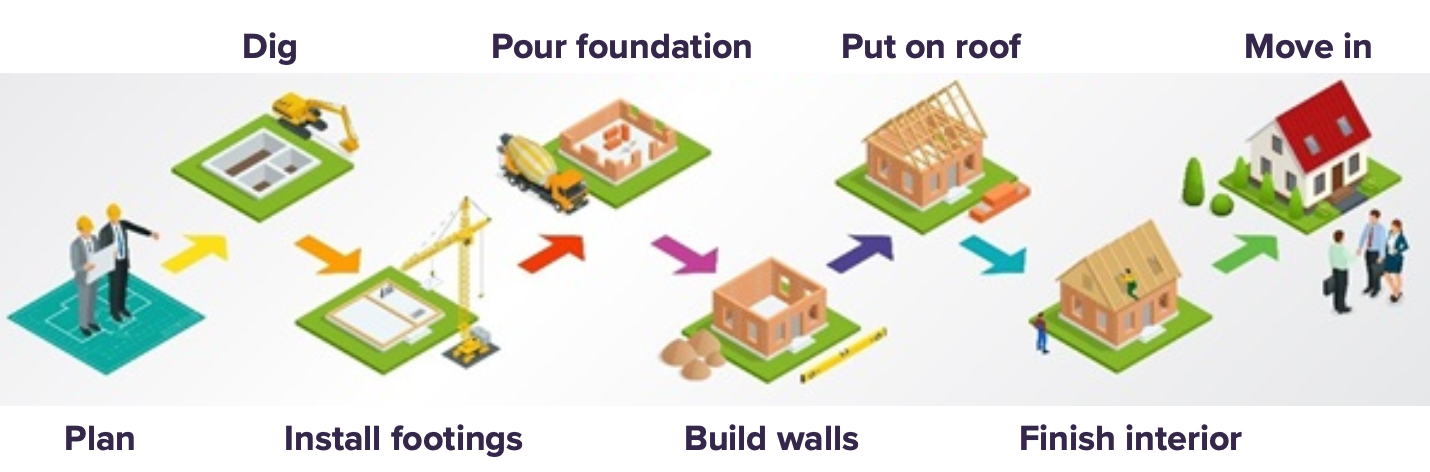
\includegraphics[keepaspectratio]{figs/fig3.png}}

\vspace{.5cm}

There's only one way to manage something so complex:

\begin{itemize}
\tightlist
\item
  \textcolor{burntorange}{Break down} the complex task into simpler
  tasks
\item
  \textcolor{burntorange}{Sequence} the tasks so that each one builds on
  prior tasks and feeds into subsequent tasks
\end{itemize}
\end{frame}

\begin{frame}{An analogy: Building a house}
\phantomsection\label{an-analogy-building-a-house-1}
A quantitative argument is built from sequencing simpler tasks

\begin{itemize}
\tightlist
\item
  \textcolor{burntorange}{Framing} the question
\item
  Building a \textcolor{burntorange}{model}
\item
  Gathering \textcolor{burntorange}{data}
\item
  Making defensible \textcolor{burntorange}{assumptions}
\item
  \textcolor{burntorange}{Probing} the model's outputs
\end{itemize}
\end{frame}

\begin{frame}{}
\phantomsection\label{section-9}
\vspace{.5cm}

\Large Is college worth it?
\end{frame}

\end{document}
